\section{Исследование и построение решения задачи}
\label{sec:Chapter3} \index{Chapter3}

\subsection{Описание иерархической структуры документа общего вида}
\label{subsec:structuredescription}

\subsection{Разработка метода построения иерархической структуры общего вида}
\label{subsec:extractmethod}

Согласно подсекции~\ref{subsec:structuredescription} дерево документа, которое необходимо построить,
является упорядоченным, а в своих узлах содержит строки текстового документа.
Для того, чтобы построить такое дерево для произвольного документа, необходимо:
\begin{enumerate}
    \item Получить упорядоченное множество строк документа;
    \item Для каждой строки найти строку-родителя, которая находится выше по иерархии, и строки-потомки, которые структурно вложены по отношению к данной строке.
\end{enumerate}
Для нахождения иерархии строк, то есть того, какая строка является предком, а какая потомком,
можно применять метод попарного сравнения строк.
Этот метод подразумевает одновременное последовательное прохождение по строкам документа и построение дерева документа.
При этом, из каждой новой рассматриваемой строки документа нужно сформировать новый узел дерева, а для этого определить место вставки узла.
При анализе документа мы опираемся на тот факт, что некоторые строки являются более значимыми,
то есть являются составными частями более значимых структурных элементов, чем другие строки.
Например, строка-заголовок документа является более значимой, чем простая текстовая строка.
Если мы умеем определять, какая из двух строк более значима, то мы сможем определить место вставки очередного узла в дерево документа.
Если строка менее значима, чем предыдущая, то нужно добавить новый лист, если же строка оказалась более значимой,
то её необходимо проходить вверх по иерархии дерева и искать строку-родителя для нахождения места вставки.
Более точно процесс построения дерева документа описывается алгоритмом~\ref{alg:treebuilding}.

\begin{algorithm}
    \hspace*{\algorithmicindent} \textbf{Input:} $L$ -- список из $N$ строк документа \\
    \hspace*{\algorithmicindent} \textbf{Output:} $T$ -- дерево документа
    \begin{algorithmic}
        \State $current\_line \gets L[0]$
        \State $T \gets make\_node(current\_line)$ \Comment{Создание из строки документа узла дерева}
        \State $current\_node \gets T$
        \State $i \gets 1$
        \While{$i < N$}
            \State $next\_line \gets L[i]$
            \State $cmp \gets compare\_lines(current\_line, next\_line)$ \Comment{Сравнение строк}
            \If{$cmp = less$} \Comment{$next\_line < current\_line$}
                \State $new\_node \gets make\_node(next\_line)$
                \State $add\_child(current\_node, new\_node)$
            \ElsIf{$cmp = greater$} \Comment{$next\_line > current\_line$}
                \If{$current\_node$ является корнем}
                    \State $new\_node \gets make\_node(next\_line)$
                    \State $T \gets new\_node$
                    \State $add\_child(new\_node, current\_node)$
                \Else
                    \State $current\_node \gets get\_parent(current\_node)$
                    \State $current\_line \gets get\_line(current\_node)$
                    \State \textbf{continue}
                \EndIf
            \Else \Comment{$next\_line = current\_line$}
                \State $parent\_node \gets get\_parent(current\_node)$
                \State $new\_node \gets make\_node(next\_line)$
                \State $add\_child(parent\_node, new\_node)$
            \EndIf
            \State $current\_line \gets next\_line$
            \State $current\_node \gets new\_node$
            \State $i \gets i + 1$
        \EndWhile
    \end{algorithmic}
    \caption{Алгоритм построения дерева документа}
    \label{alg:treebuilding}
\end{algorithm}

Согласно указанному алгоритму, основная задача, которая должна быть решена -- это определение для пары строк документа, какая из них является более значимой.
Эта задача не является полностью формализованной, так как у документов разных типов оформление сильно различается.
Однако есть некоторые общие правила по выделению структурированных элементов в виде заголовков и списков.
Таким образом, для решения данной задачи можно применить методы машинного обучения.

Для применения машинного обучения необходимо составить набор данных, на которых можно обучаться.
Так как поставленная задача еще никем не решалась, создание набора данных становится одной из подзадач, которые надо решить.
При этом, надо принять во внимание тот факт, что документы в наборе данных должны различаться по структуре, оформлению и предметной области.
Процесс разметки не является очевидным, поэтому для создания набора размеченных данных требуется создать программную систему,
которая бы позволила размечать (сравнивать) пары строк так, как это делается в алгоритме построения дерева документа.
На основании созданного и размеченного набора документов далее можно обучить алгоритм машинного обучения,
который позволил бы сравнивать строки документа по значимости, а значит и находить место вставки каждой строки-узла в итоговое дерево документа.

Обобщая всё вышесказанное, для решения задачи построения дерева документа предлагается следующая последовательность действий:
\begin{enumerate}
    \item Сформировать набор документов с разным оформлением и предметной областью;
    \item Создать систему разметки, позволяющую динамически создавать задания для сравнения строк документа;
    \item Организовать получение упорядоченного списка строк из документов с дополнительной информацией, необходимой для системы разметки;
    \item Применить алгоритм машинного обучения на размеченных данных для сравнения строк документа;
    \item Основываясь на списке выделенных из документа строк, а также обученном алгоритме сравнения строк, построить дерево документа согласно описанному алгоритму~\ref{alg:treebuilding}.
\end{enumerate}

\subsubsection{Описание набора данных}

В набор данных включены несколько типов документов, написанных на разных языках:
\begin{itemize}
    \item Нормативно-правовые акты на русском языке;
    \item Нормативно-правовые акты на армянском языке;
    \item Научные статьи на английском языке;
    \item Финансовые документы на английском и французском языках.
\end{itemize}

Основная информация о документах представлена в таблице~\ref{tab:dataset}.
\begin{table}
    \begin{center}
        \begin{tabular}{|p{4cm}|p{3cm}|p{5cm}|p{2.5cm}|}
            \hline
            \textbf{Предметная область} & \textbf{Язык} & \textbf{Источник} & \textbf{Количество документов} \\
            \hline
            \hline
            Нормативно-правовые акты & русский & Официальный портал правовой информации\tablefootnote{\url{http://publication.pravo.gov.ru/}} & 20 \\
            \hline
            Нормативно-правовые акты & армянский & Информационная система\tablefootnote{\url{https://www.arlis.am/}} и электронное правительство\tablefootnote{\url{https://www.e-gov.am/en/}} Республики Армения & 20 \\
            \hline
            Научные статьи & английский & Архив научных статей с открытым доступом\tablefootnote{\url{https://arxiv.org/}} & 20 \\
            \hline
            Финансовые документы & английский, французский & Сайт соревнований FinTOC-2021\tablefootnote{\url{http://wp.lancs.ac.uk/cfie/fintoc2021/}} & 10 \\
            \hline
        \end{tabular}
    \end{center}
    \caption{Описание набора данных}
    \label{tab:dataset}
\end{table}

Все документы представлены в формате PDF как с текстовым слоем, так и без него.
Среди них присутствуют документы разного оформления: одноколоночные и двухколоночные, написанные шрифтом разного размера, в некоторых документах присутствуют нетекстовые документы такие как печати, таблицы, изображения.
Примеры страниц документов разных типов представлены на рисунке~\ref{fig:documentexamples}.

\begin{figure}[h]
    \centering
    \begin{minipage}[h]{0.22\linewidth}
    \center{\frame{
\includegraphics[height=0.22\textheight]{img/russian}} \\ а) НПА на русском}
    \end{minipage}
    \begin{minipage}[h]{0.22\linewidth}
    \center{\frame{
\includegraphics[height=0.22\textheight]{img/armenian}} \\ б) НПА на армянском}
    \end{minipage}
    \begin{minipage}[h]{0.22\linewidth}
    \center{\frame{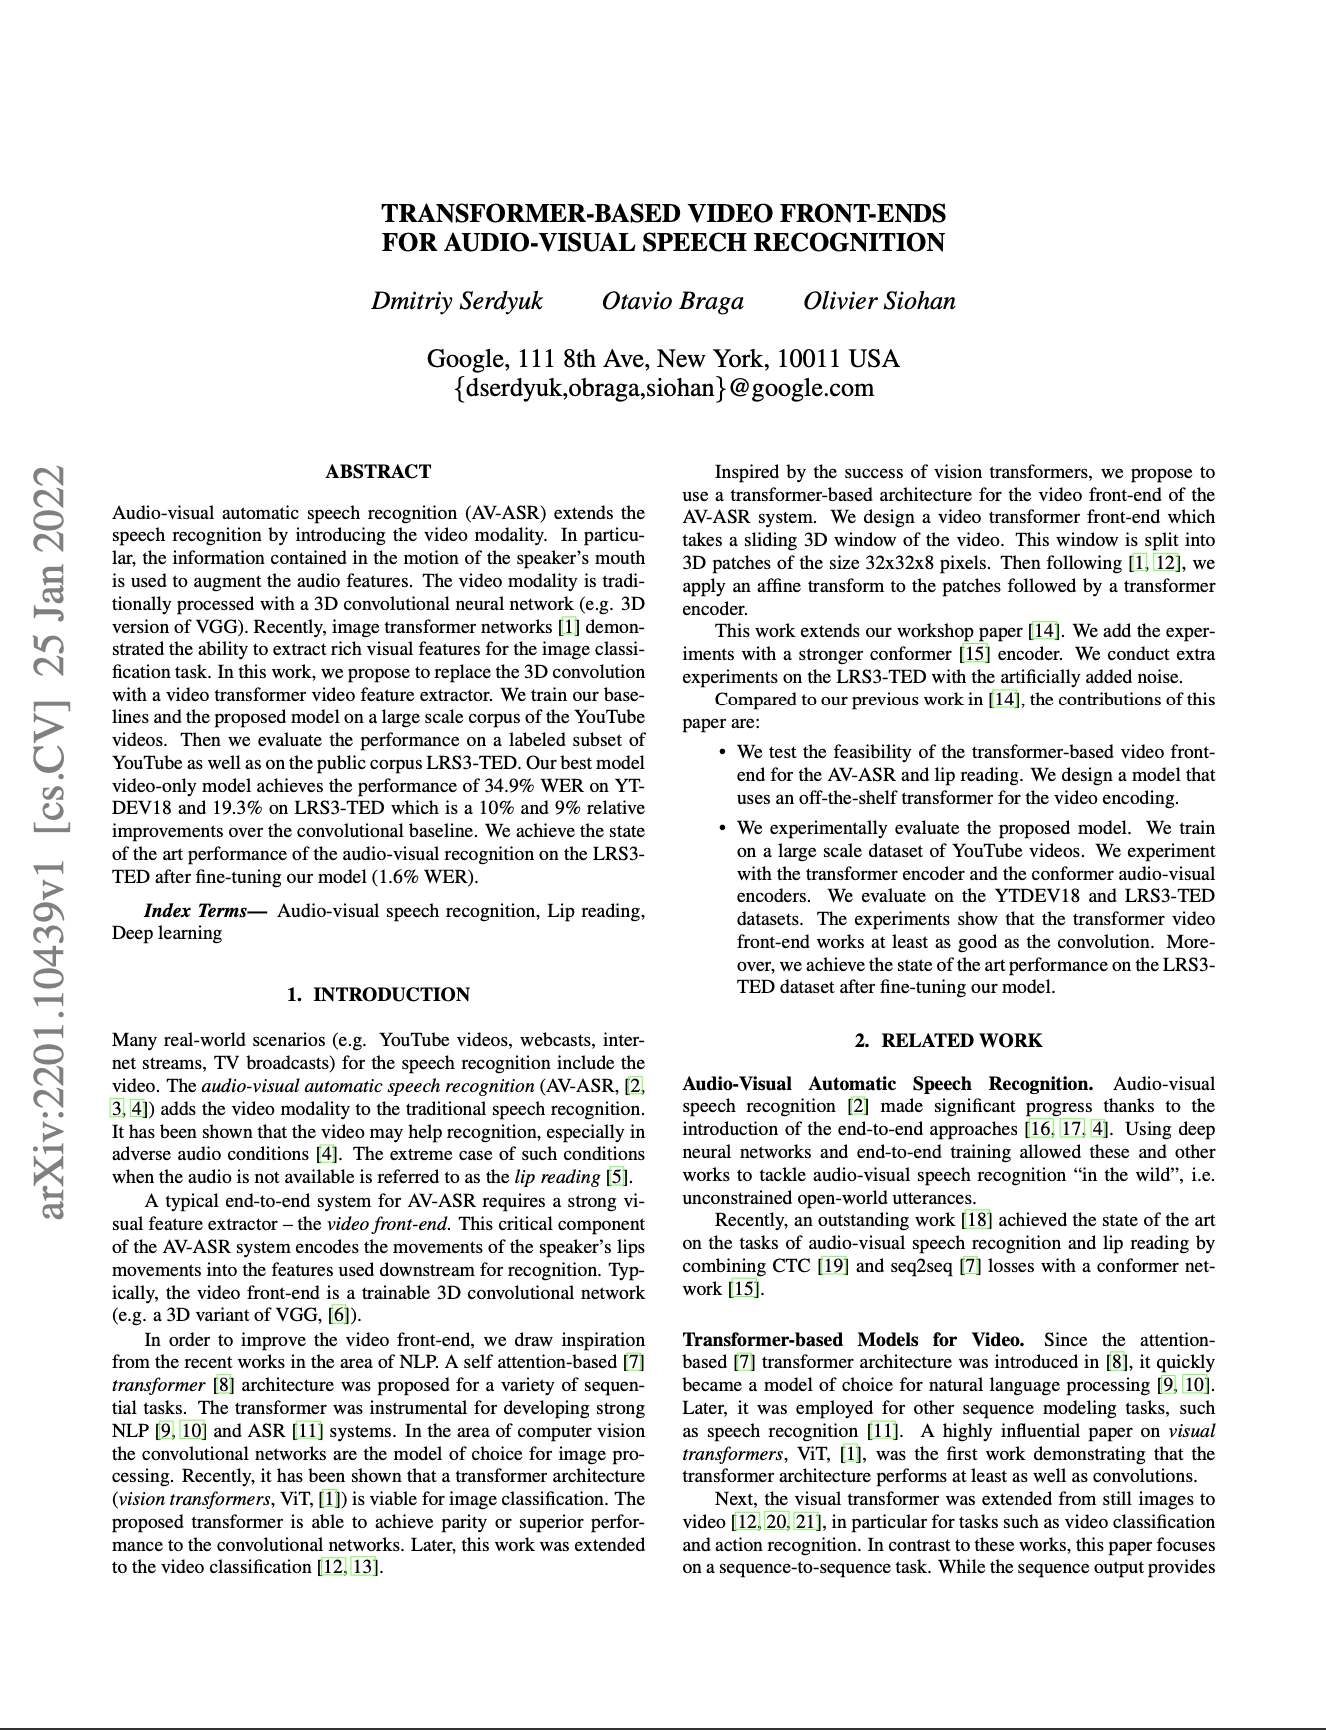
\includegraphics[height=0.22\textheight]{img/article}} \\ в) Научная статья}
    \end{minipage}
    \begin{minipage}[h]{0.22\linewidth}
    \center{\frame{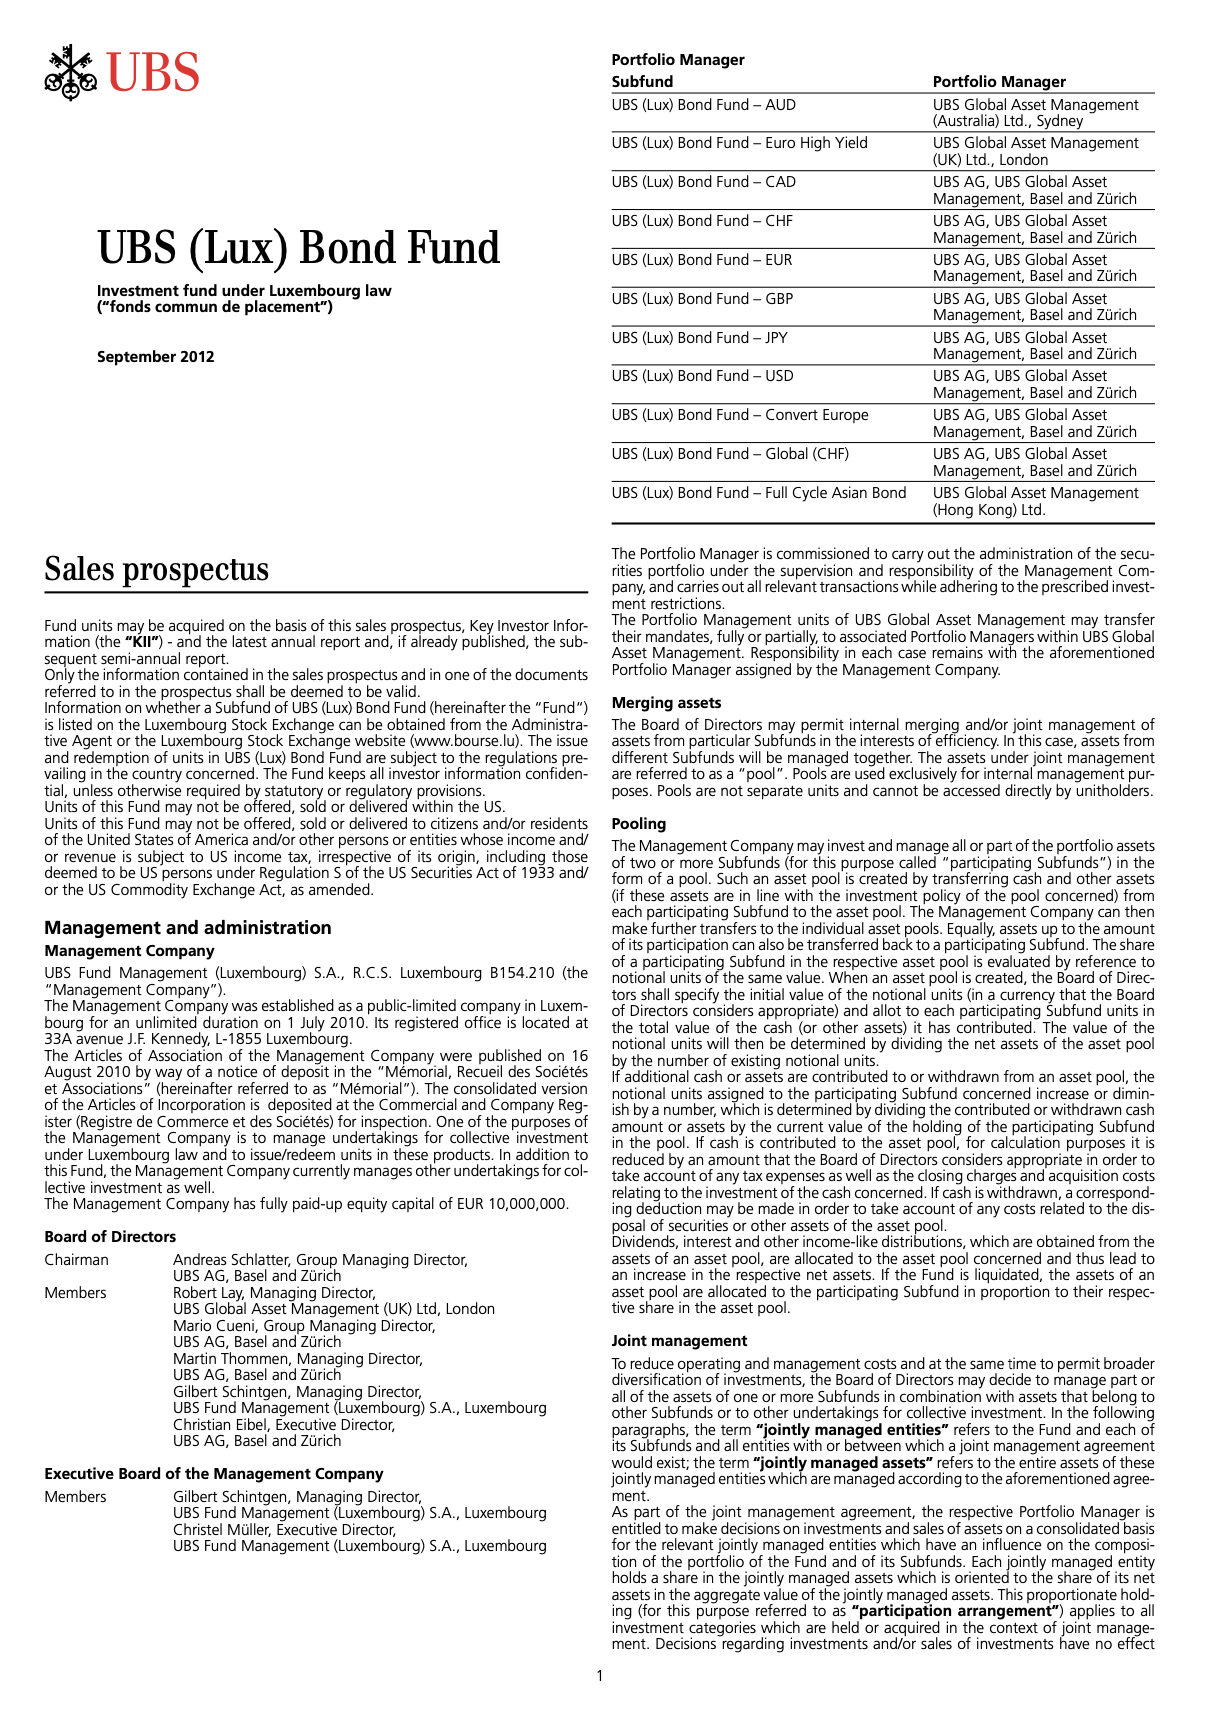
\includegraphics[height=0.22\textheight]{img/fintoc}} \\ г) Финансовый документ}
    \end{minipage}
    \caption{Примеры страниц документов из набора данных}
    \label{fig:documentexamples}
\end{figure}

\todo[inline]{Описать поподробнее и мб добавить статистики}

\subsubsection{Система разметки}

Поставленная задача подразумевает сравнение двух строк между собой.
Для разметчика эту задачу можно поставить как задачу классификации изображений:
\begin{enumerate}
    \item Система выдаёт разметчику изображение, состоящее из двух страниц документа, на каждой из страниц выделена одна из строк;
    \item Разметчик определяет, какая из выделенных строк <<важнее>>, классифицируя таким образом изображение.
\end{enumerate}

Для того, чтобы процесс разметки походил на процесс выполнения алгоритма построения дерева документа, необходимо уметь решать динамически, какую пару строк сравнивать следующей.
А для этого в системе разметки должен быть прописан алгоритм, похожий на описанный выше алгоритм построения дерева (см. алгоритм~\ref{alg:treebuilding}).
Кроме того, нужно уметь каким-то образом выделять строки на страницах документа.
Для документов в формате PDF можно сохранять страницы как изображения, а для строк находить координаты рамок, ограничивающих текст строки (bounding boxes).
Таким образом, для системы разметки документ достаточно представить как список прочитанных строк со следующей информацией:
\begin{itemize}
    \item устойчивый уникальный идентификатор строки;
    \item путь до изображения страницы с данной строкой;
    \item координаты ограничивающей рамки для строки.
\end{itemize}
При наличии такой информации можно создавать изображение, состоящее из двух страниц документа, на каждой их которых одна строка обведена в рамку.
Уникальный идентификатор строки нужен для навигации по списку строк при выборе очередной пары строк, которые нужно сравнить.

Обобщая всё перечисленное, система разметки должна предоставлять следующие возможности:
\begin{itemize}
    \item Формирование входных данных для разметки, то есть получение из документа списка строк с
    идентификатором, путём до изображения страницы и координатами ограничивающей рамки, а также сохранение страниц документа как отдельных изображений.
    \item Формирование изображений, которые нужно классифицировать.
    Изображения формируются обведением на изображениях страниц нужных строк в рамки, а также соединением две страницы в одно изображение.
    \item Формирование заданий для разметчика, т. е. последовательный проход по полученным из документа строкам и в соответствии с алгоритмом построения дерева и результатами разметки предыдущих строк формирование следующих заданий для разметки.
    Задания для разметки получаются с помощью формирования изображений.
    \item Пользователь (разметчик) должен иметь возможность взаимодействовать с системой разметки и сохранять результаты своего труда.
\end{itemize}

Программная реализация такой системы описана в главе~\ref{sec:Chapter4}.
Предлагается ввести 4 класса, на которые нужно классифицировать изображения: вторая строка <<меньше>> (less), <<больше>> (greater) или <<равна>> (equal) первой, либо одна из строк не является текстовой строкой, т.е. <<другое>> (other).
Эти классы, а также правила, по которым разметчик должен снабжать метками изображения, описаны в подсекции~\ref{subsubsec:labelingprocess}.
Здесь же схематично приведён алгоритм~\ref{alg:labeling}, по которому в зависимости от предыдущих результатов разметки формируются новые задания.

\begin{algorithm}[h]
    \hspace*{\algorithmicindent} \textbf{Input:} $L$ -- список строк документа с дополнительной информацией, \\
    \hspace*{\algorithmicindent} $T$ -- список размеченных заданий из $id_1,~id_2,~label$, \\
    \hspace*{\algorithmicindent} где $id_1,~id_2$ -- индексы сравниваемых строк в списке $L$, $label$ -- метка \\
    \hspace*{\algorithmicindent} \textbf{Output:} $new\_task$ -- новое задание для разметки
    \begin{algorithmic}
        \State $last\_label \gets get\_last\_label(T)$ \Comment{Метка для последнего задания}
        \State $last\_id_1, last\_id_2 \gets get\_last\_ids(T)$ \Comment{Номера строк в списке $L$ из задания}
        \If{$last\_label = other$}
            \State $line \gets find\_line(T)$ \Comment{Поиск строки в заданиях с меткой $\neq other$}
            \State $new\_task \gets make\_task(line, last\_id_2 + 1)$ \Comment{Формирование задания}
        \ElsIf{$last\_label = greater$}
            \State $line \gets find\_line(last\_id_1, T)$ \Comment{Поиск строки > строки с номером $last\_id_1$}
            \State $new\_task \gets make\_task(line, last\_id_2)$ \Comment{Формирование задания}
        \Else \Comment{$last\_label = less$ или $last\_label = equal$}
            \State $new\_task \gets make\_task(last\_id_2, last\_id_2 + 1)$ \Comment{Формирование задания}
    \end{algorithmic}
    \caption{Алгоритм формирования задания для разметки}
    \label{alg:labeling}
\end{algorithm}



\subsubsection{Процесс разметки документов}
\label{subsubsec:labelingprocess}

Для того, чтобы процесс разметки всего набора данных был осмысленным и согласованным с поставленной задачей, а результаты отностительно однозначными, необходимо провести некоторую предварительную работу:
\begin{enumerate}
    \item Сформулировать правила правильной разметки (манифест);
    \item Дать нескольким разметчикам небольшое количество заданий для разметки и получить результаты;
    \item Сравнить результаты и в случае грубых несоответствий вернуться к первому шагу и начать всё сначала, пересмотрев манифест.
\end{enumerate}
Если разметчики достигли определённого уровня согласованности при выполнении задания, значит правила разметки адекватны и можно приступать к разметке всего набора данных.

Таким образом, для осуществления процесса разметки нужно составить манифест и выбрать метрику для сравнения результатов.

\paragraph{Правила разметки.} Строго сформулированные правила разметки вкратце описываются следующим образом:
\begin{itemize}
    \item Задание состоят из пар изображений страниц одного документа, на каждой из страниц одна из строк выделена.
    Нужно определить, больше, меньше или равна вторая строка документа первой строке и присвоить одну из меток: <<greater>>, <<less>>, <<equal>>, <<other>>.
    \item Строки документа могут иметь разное выделение, для которого могут использовать отступ, выравнивание; полужирный, подчёркнутый или курсивный шрифт; текст из заглавных букв, префиксы для элементов списка в начале строки.
    \item Строки считаются равными (equal) по уровню вложенности, если они являются составляющими одинаково (похожим образом) выделенных структурных элементов. Например, заголовки двух глав, два элемента одного списка, две строки одного текстового блока.
    \item Вторая строка меньше первой (less), если первая строка – заголовок (сильно выделена), а вторая – список или текст; либо первая строка – список, а вторая текст; либо первая строка визуально более выделена, чем вторая (жирностью, отступом и т. д.); либо это многоуровневый список.
    Для greater всё аналогично с точностью до наоборот.
    \item Тип <<other>> выбирается, когда хотя бы одна из строк является сноской (номером страницы, и т.д.), либо рукописным текстом, либо вообще не текстом (картинка, текстовый блок из нескольких строк и т. д.)
\end{itemize}

\paragraph{Метрика для сравнения результатов разметки.} Для сравнения древовидных структур документов (например, содержания) в нескольких соревнованиях~\cite{doucet2013icdar,fintoc2019,fintoc2020,el2021financial} использовалась функция следующего вида:
\[ precision = \frac{correct}{correct + added + mismatch} \]
\[ recall = \frac{correct}{correct + missed + mismatch} \]
\[ F1 = \frac{2 \cdot precision \cdot recall}{precision + recall}, \]
где
\begin{itemize}
    \item $correct$ --
    \item $mismatch$ --
    \item $added$ --
    \item $missed$ --
\end{itemize}

\subsubsection{Обучение алгоритма сравнения строк}


\subsection{Разработка метода использования иерархической структуры общего вида}
\label{subsec:usemethod}


\subsection{Оценку качества реализованного метода}
\label{subsec:evaluation}